\documentclass{beamer}
\usepackage{ctex, hyperref}
\usepackage[T1]{fontenc}

% other packages
\usepackage{latexsym,amsmath,xcolor,multicol,booktabs,calligra}
\usepackage{graphicx,pstricks,listings,stackengine}

\author{\href{}{communication Management ara::com}}
\institute{\href{}{Automotive Mechatronics Engineering Department}}
\title{Adaptive AutoSAR Graduation Project}
\subtitle{AA , ara::com}
\date{}
\usepackage{Amr_Beamer}

% defs
\def\cmd#1{\texttt{\color{red}\footnotesize $\backslash$#1}}
\def\env#1{\texttt{\color{blue}\footnotesize #1}}	
\definecolor{deepblue}{rgb}{0,0,0.5}
\definecolor{deepred}{rgb}{0.6,0,0}
\definecolor{deepgreen}{rgb}{0,0.5,0}
\definecolor{halfgray}{gray}{0.55}

\lstset{
	basicstyle=\ttfamily\small,
	keywordstyle=\bfseries\color{deepblue},
	emphstyle=\ttfamily\color{deepred},   % Custom highlighting style
	stringstyle=\color{deepgreen},
	numbers=left,
	numberstyle=\small\color{halfgray},
	rulesepcolor=\color{red!20!green!20!blue!20},
	frame=shadowbox,
}


\begin{document}
	
	\kaishu
	\begin{frame}
		\titlepage
		\begin{figure}
			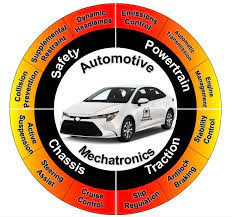
\includegraphics[scale=0.2]{pic/depart.jpg} 
		\end{figure}
	\end{frame}
	
	\begin{frame}
		\tableofcontents[sectionstyle=show,subsectionstyle=show/shaded/hide,subsubsectionstyle=show/shaded/hide]
	\end{frame}
	
	
	\section{Classic Autosar}
	
	\begin{frame}{Introduction}
		\begin{figure}
			\centering
			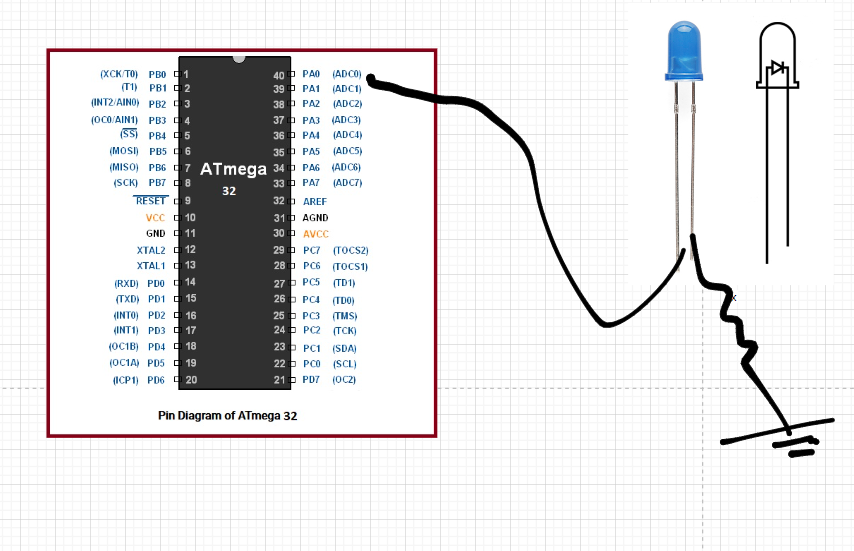
\includegraphics[width = 9cm, height = 4cm]{pic/led_at.PNG}
		\end{figure}
		\begin{itemize}
			\item NonAutoSAR Application: Toggle the led on pin A0 each 1 sec.
		\end{itemize}
	\end{frame}
	
	\begin{frame}{Code}
		\begin{figure}
			\centering
			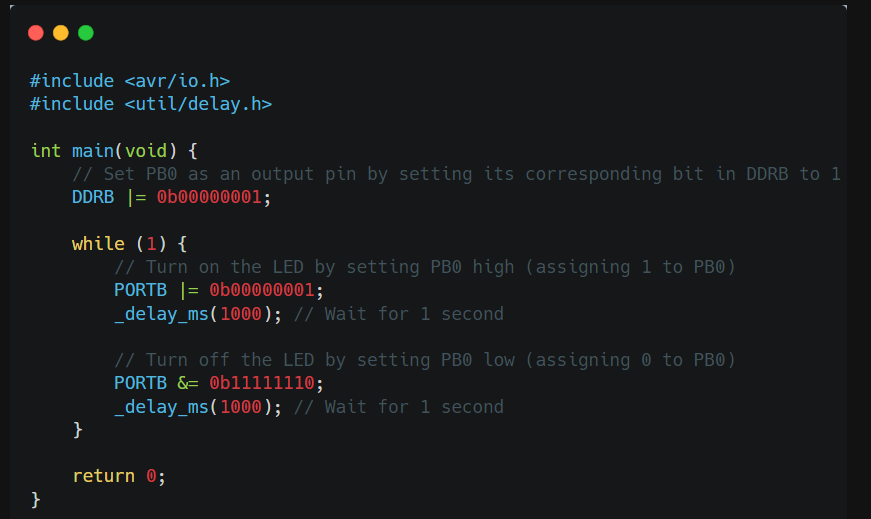
\includegraphics[width = 9cm, height = 4cm]{pic/code_led.PNG}
		\end{figure}
		\begin{itemize}
			\item Datasheet: 
			\begin{itemize}
				\item	1- specify pin to be OUTPUT
				\item	2- generative 5v to be OUTPUT HIGH 
			\end{itemize}
			
		\end{itemize}
		
	\end{frame}
	
	\begin{frame}{Imagine}
		\begin{figure}
			\centering
			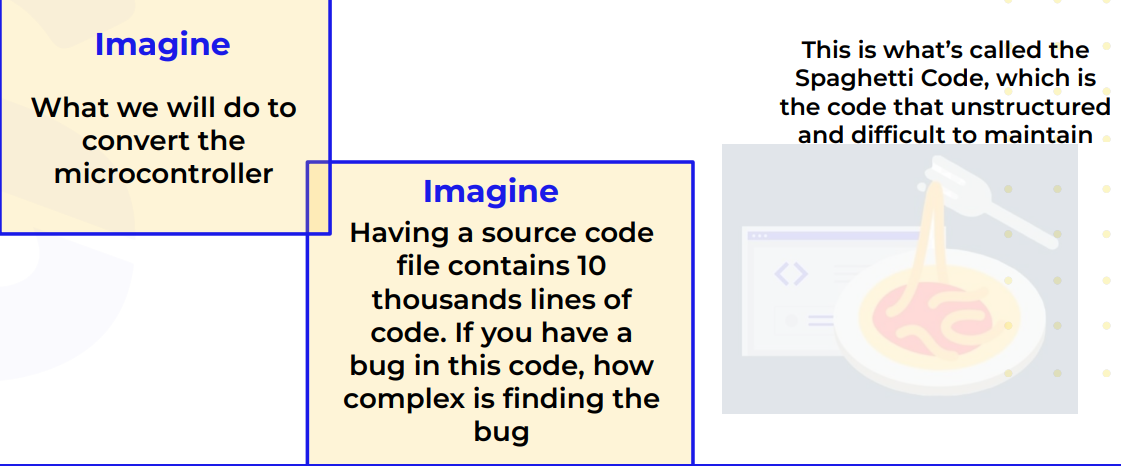
\includegraphics[width = 9cm, height = 4cm]{pic/imagine.PNG}
		\end{figure}	
	\end{frame}
	
	\begin{frame}{Layered Archiecture}
		\begin{figure}
			\centering
			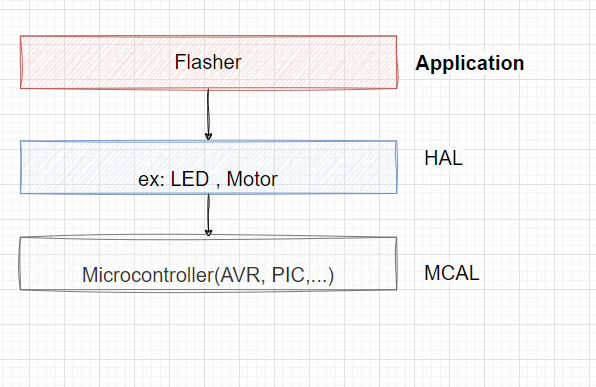
\includegraphics[width = 9cm, height = 4cm]{pic/laye.PNG}
		\end{figure}	
	\end{frame}
	
	\begin{frame}{Layered Archiecture}
		\begin{figure}
			\centering
			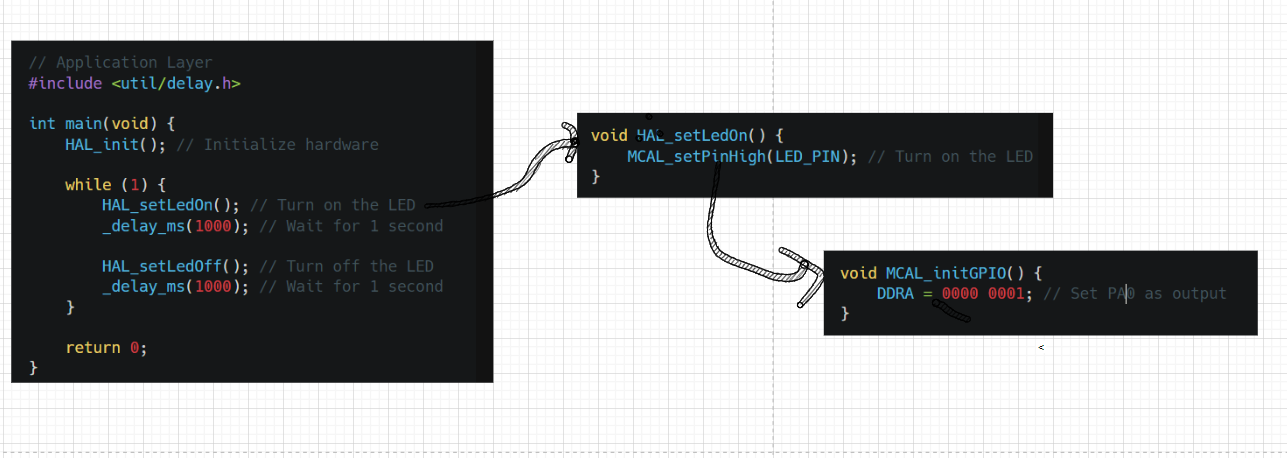
\includegraphics[width = 11cm, height = 6cm]{pic/lay.PNG}
		\end{figure}	
	\end{frame}		

	\section{Automotive Industry Transformation}
	
	\begin{frame}{Today's Automotive System}
		\begin{figure}
			\centering
			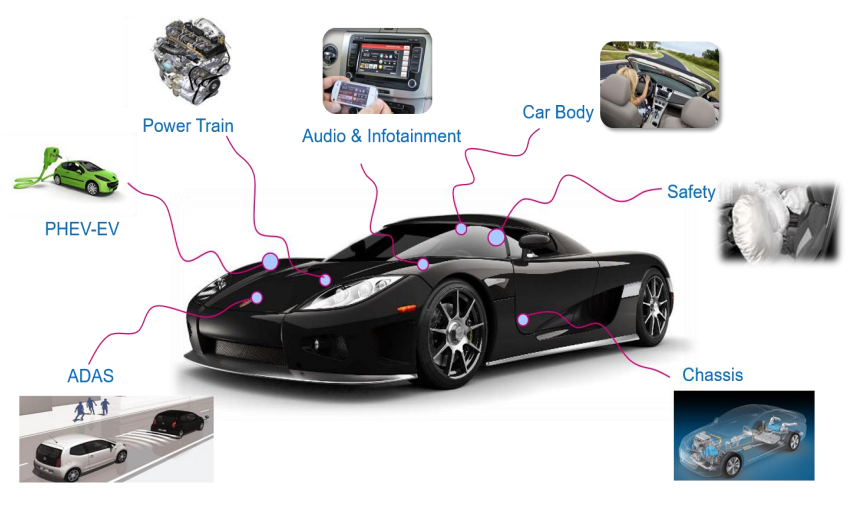
\includegraphics[width = 9cm, height = 4cm]{pic/today.PNG}
		\end{figure}
	\end{frame}
	
		\begin{frame}{PTS}
		\begin{figure}
			\centering
			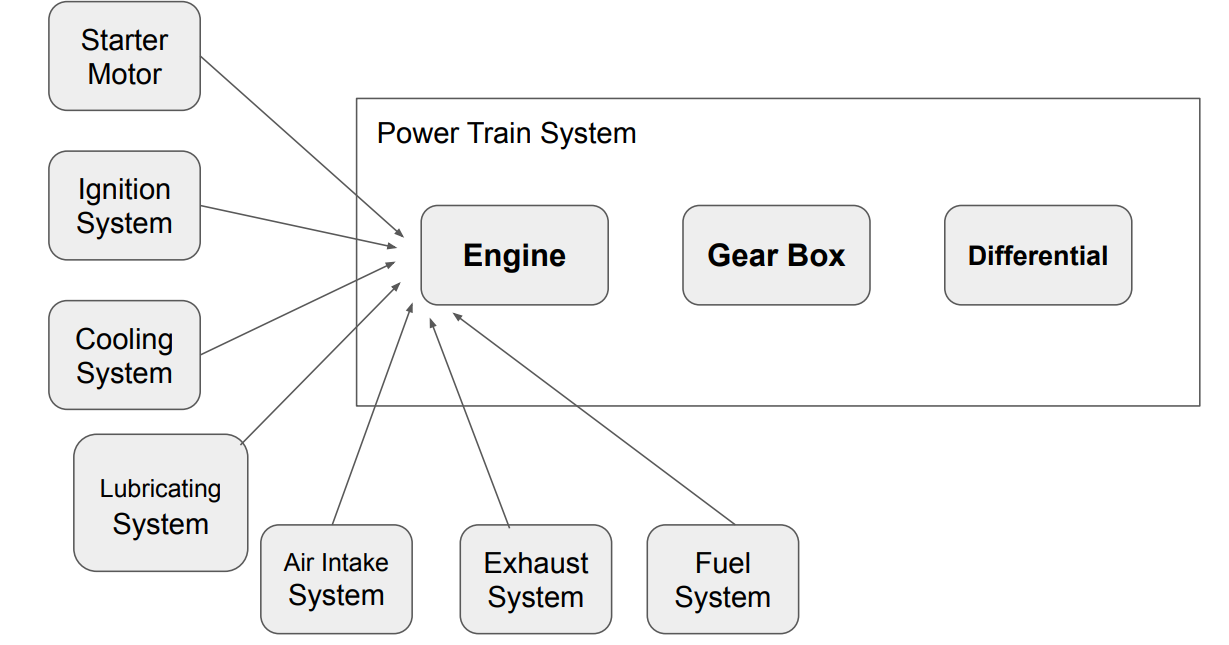
\includegraphics[width = 9cm, height = 4cm]{pic/PTS.PNG}
		\end{figure}
		
		\begin{itemize}
			\item Each System inside PTS System within other Automotive system has at least one ECU with its own layered Architecture.
			\item	100 million lines
		\end{itemize}
	\end{frame}
	
	\begin{frame}{Lines Of code}
		\begin{figure}
			\centering
			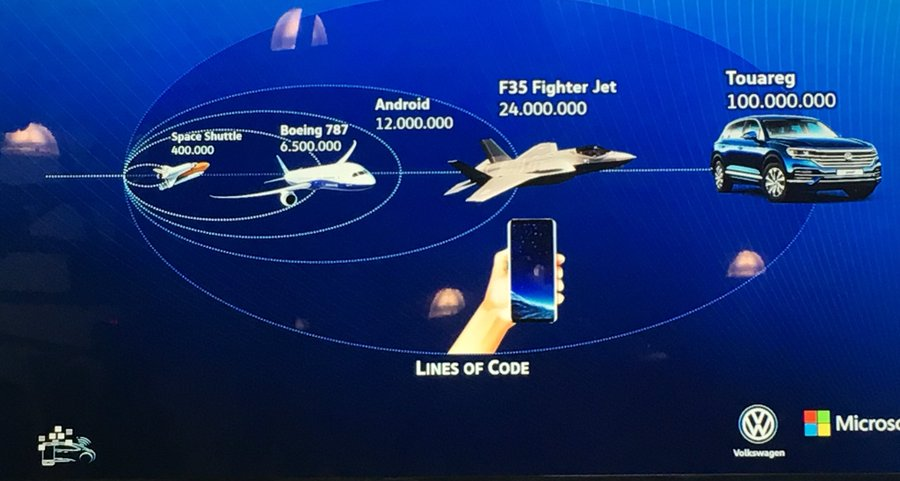
\includegraphics[width = 12cm, height = 6cm]{pic/lines.jpg}
		\end{figure}
	\end{frame}
	
		\begin{frame}{CP Architecture}
			\begin{figure}
				\centering
				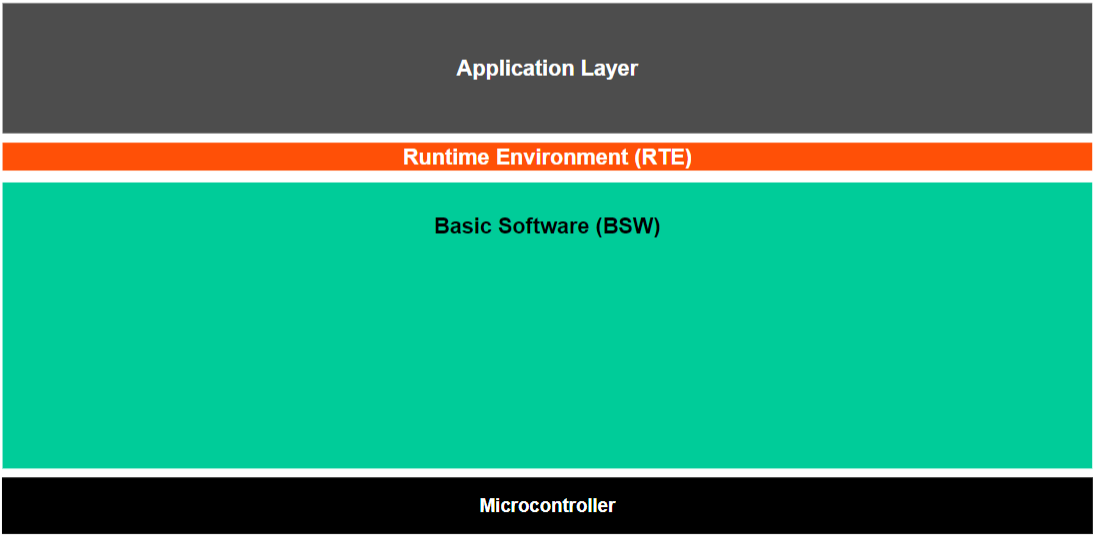
\includegraphics[width = 9cm, height = 4cm]{pic/BSW.png}
			\end{figure}
		\end{frame}

		\begin{frame}{CP Architecture}
			\begin{figure}
				\centering
				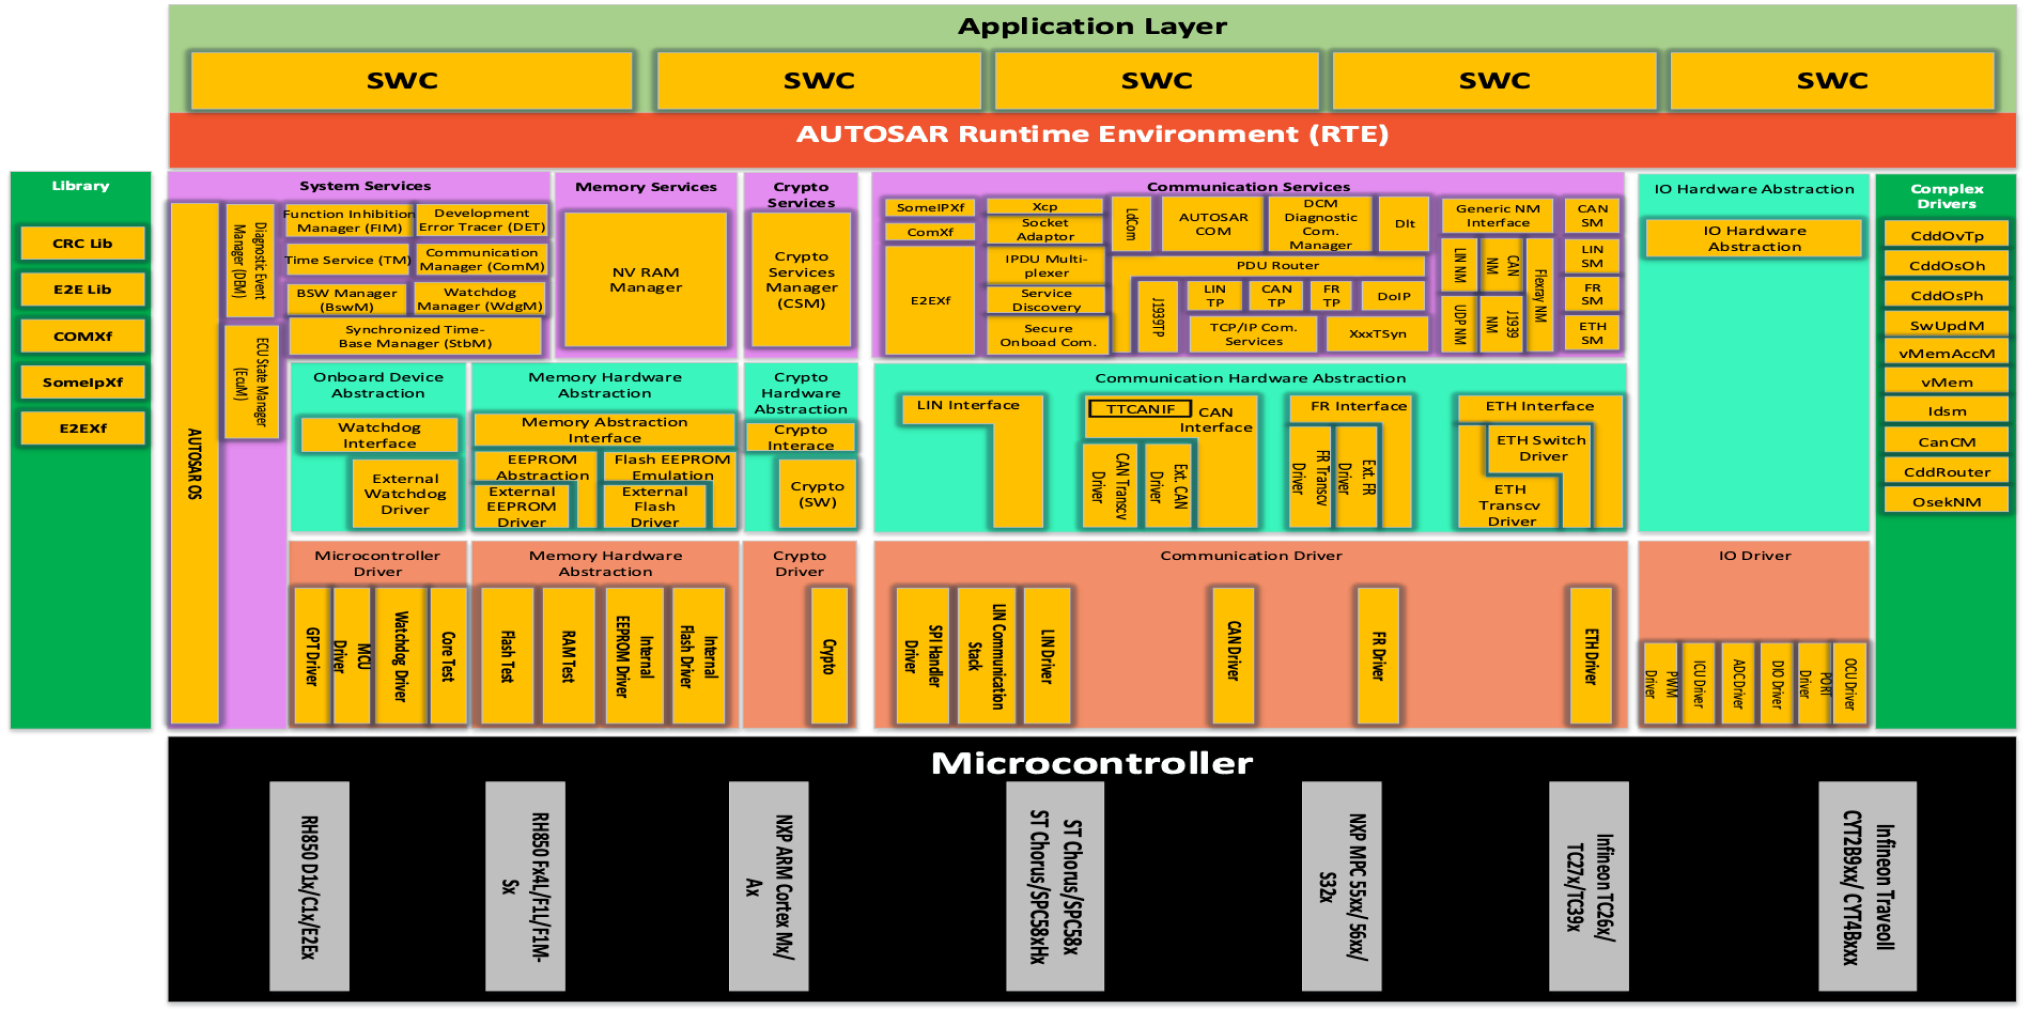
\includegraphics[width = 12cm, height = 7cm]{pic/classic-platform-bsw-introduction.png}
			\end{figure}
		\end{frame}	
	

	
	\section{Impact on MCU Design}
		\begin{frame}{Vehicle Network Applications}
			\begin{figure}
				\centering
				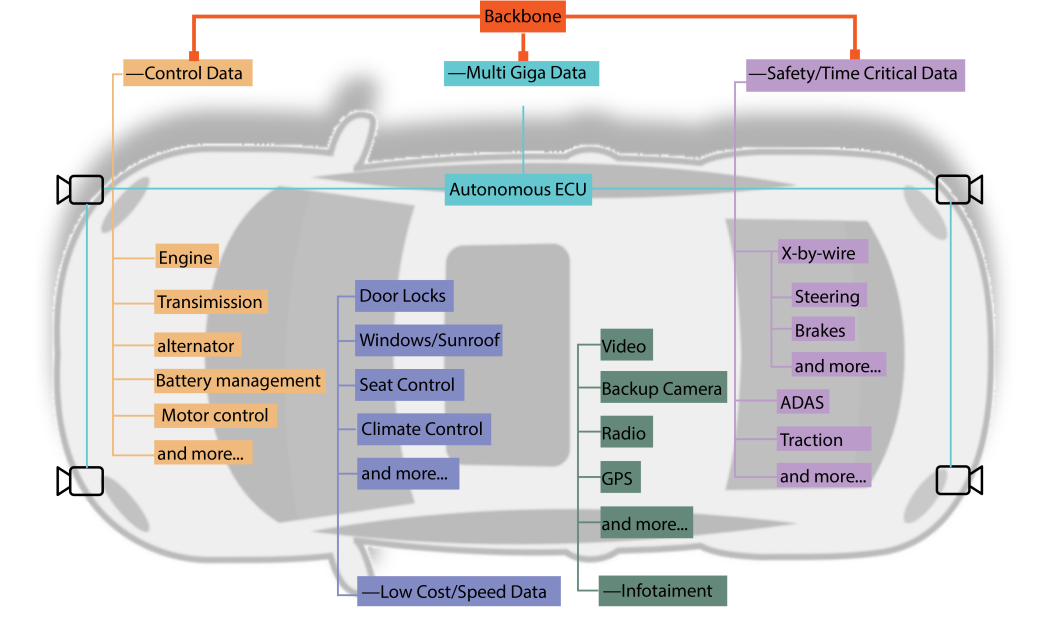
\includegraphics[width = 9cm, height = 4cm]{pic/network_data.PNG}
				\label{Vehicle Network }
			\end{figure}
			
			\begin{itemize}
				\tiny
				\item Safety/Time Critical Data: Requires relative high speed > 10Mb/s with good time synchronization and redundancy.
				\item Control Data: General Purpose for transporting data from one system to another, generally packet data. Gateways
				\item Backbone: General Purpose for transporting data from one system to a another, generally packet data. Gateways
				\item Infotainment:streaming audio/video data critical. Requires good time-sync and control data, high speed > 25Mb/s
				\item Multi Giga Data:Currently very high Bandwidth for point to point networks specialized for uncompressed video in AI
				\item Low cost/speed LOW: As cheap as possible for slow speed non-safety control: door switches, lighting, HVAC control.		
			\end{itemize}		
		\end{frame}
		
				
		\begin{frame}{HW Requirements}
			\begin{figure}
				\centering
				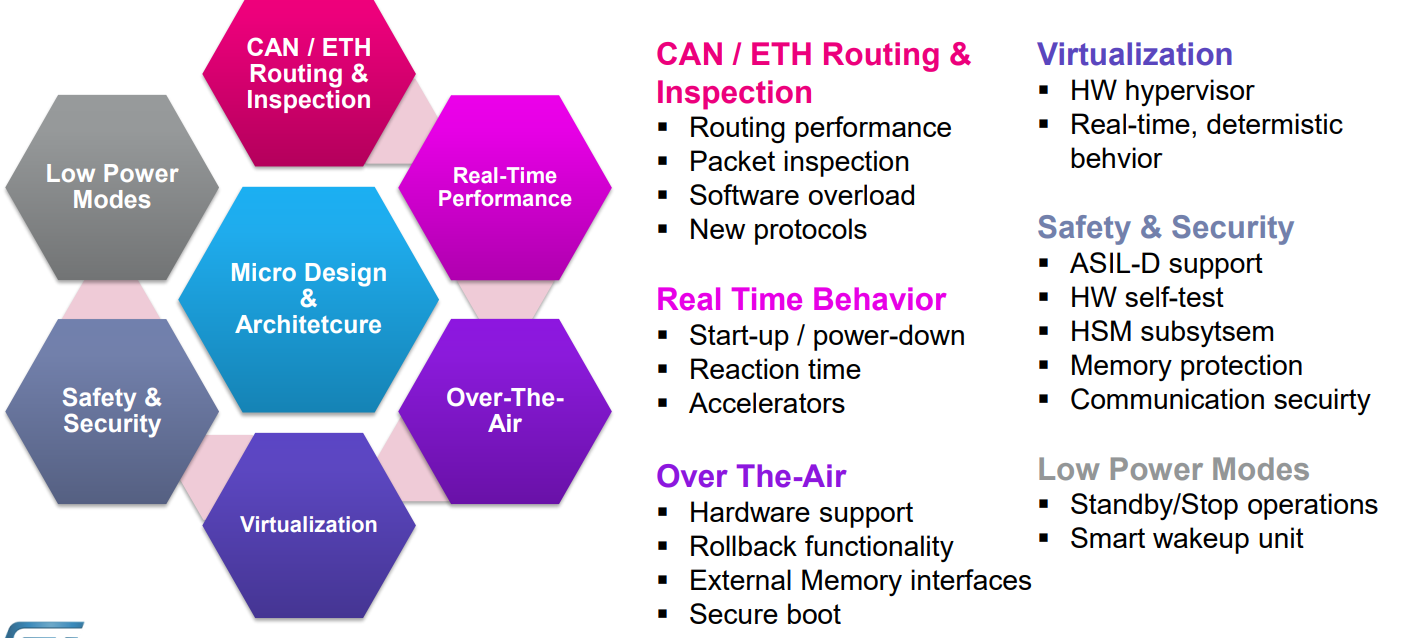
\includegraphics[width = 12cm, height = 7cm]{pic/Impact.PNG}
			\end{figure}
		\end{frame}	
		
		\begin{frame}{HW Requirements}
			\begin{figure}
				\centering
				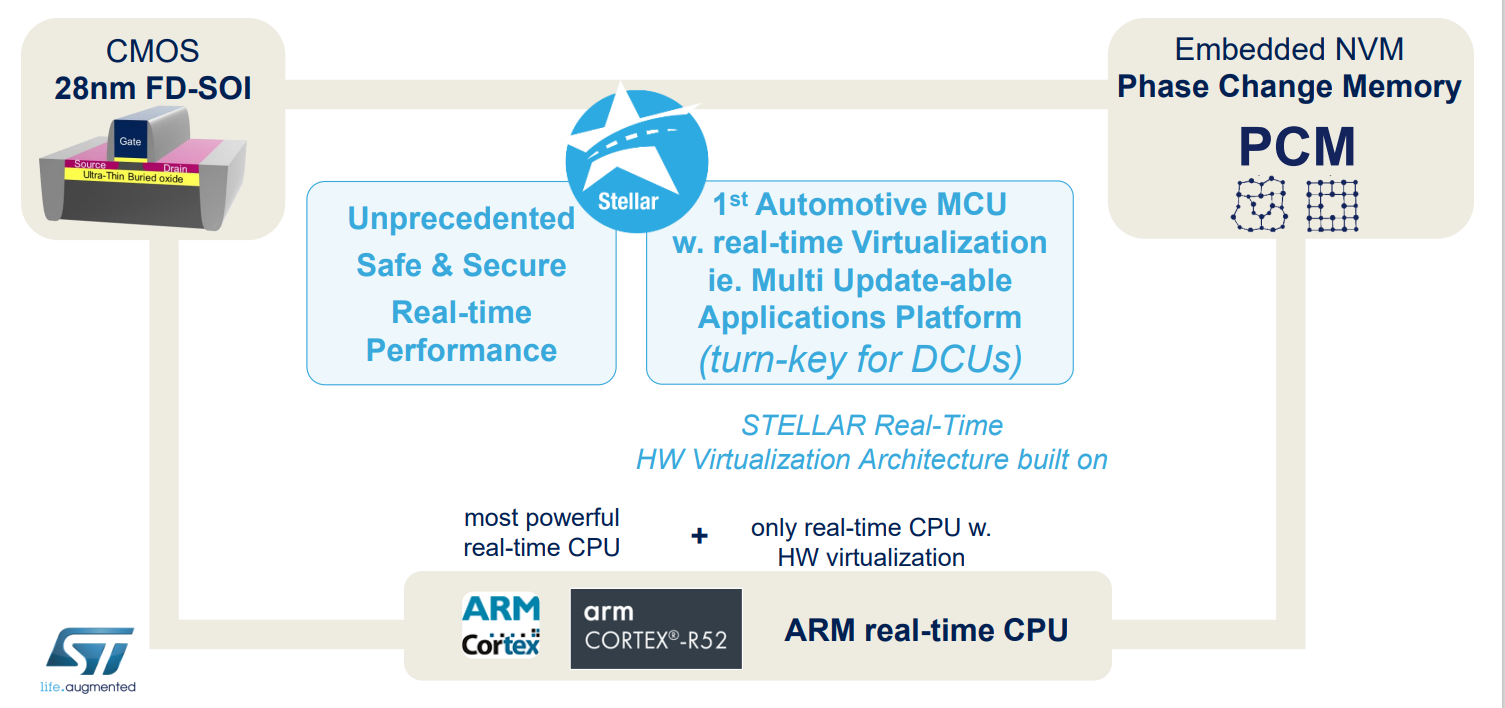
\includegraphics[width = 12cm, height = 7cm]{pic/silicon.PNG}
			\end{figure}
		\end{frame}	
		
		\begin{frame}{HW Capabilities}
			\begin{figure}
				\centering
				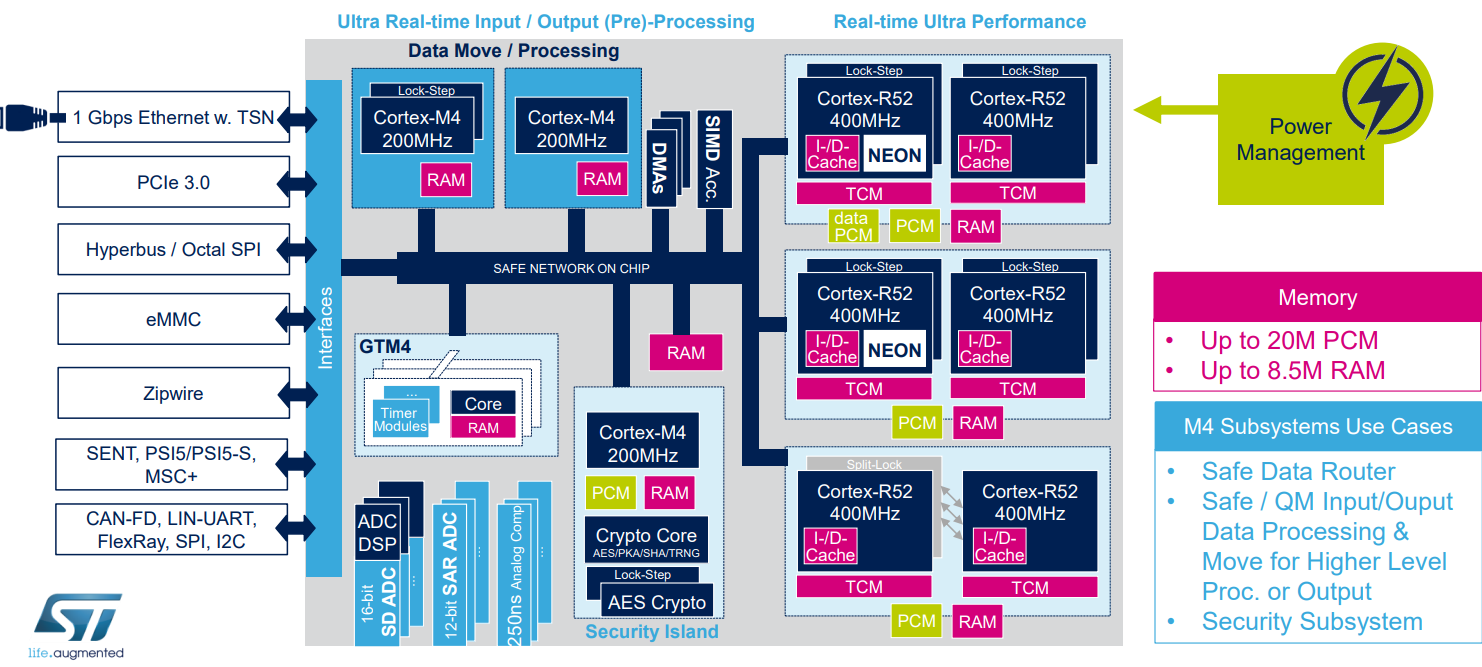
\includegraphics[width = 10cm, height = 5cm]{pic/real.PNG}
			\end{figure}
		\end{frame}	
		
	\section{Exploring AP}
		\begin{frame}{Adaptive Autosar AP}
			\begin{figure}
				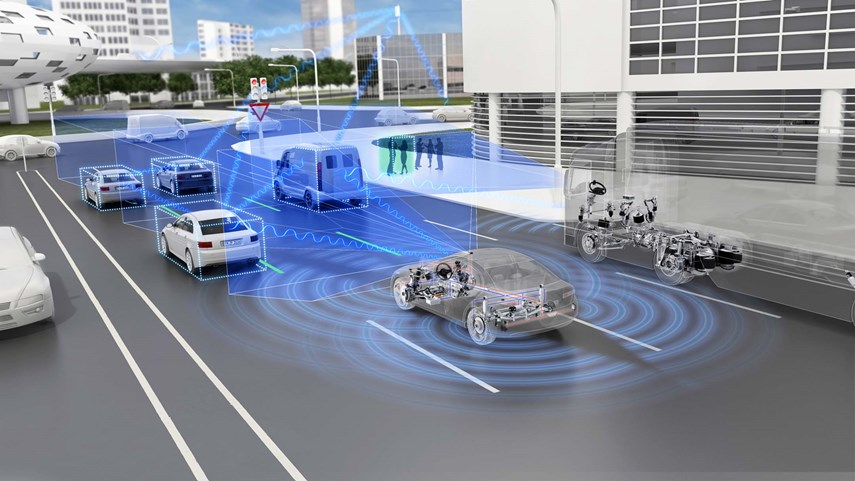
\includegraphics{pic/trends.jpg}
			\end{figure}
					
			\begin{flushright}
			\tiny
			New functionalities such as environment perception, autonomous driving, vehicle connectivity and Car as a Service(CaaS), many new functionalities and also many complexities have introduced a new set of problems to the electrical/electronic (E/E) architecture.
			\end{flushright}			
		\end{frame}

		

		\begin{frame}{Architecture}
			\begin{figure}
				\centering
				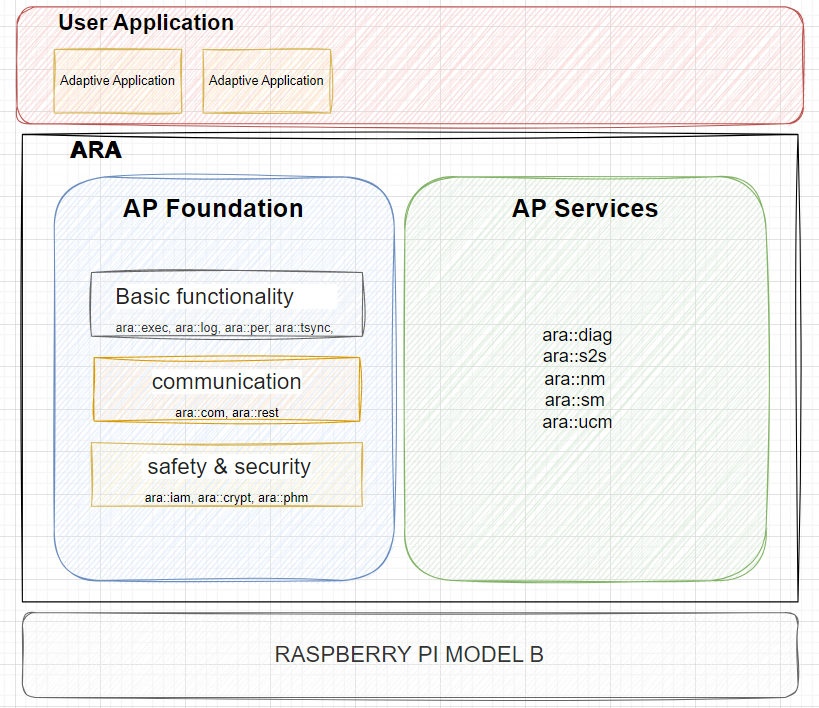
\includegraphics[width = 9cm, height =6 cm]{pic/adaptiv_simp.PNG}
			\end{figure}
		\end{frame}
		
		\begin{frame}{Adaptive Will Not Replace classic}
			\begin{figure}
				\centering
				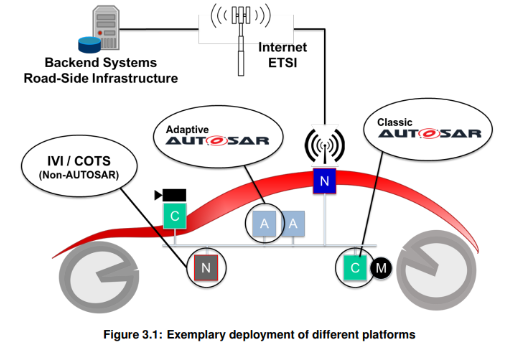
\includegraphics[width = 10cm, height = 5cm]{pic/cp_ad.PNG}
			\end{figure}
		\end{frame}
		
		
	\section{Conclusion}
		\begin{frame}{Conclusion}
			\begin{itemize}
				\item Adaptive AUTOSAR comes to life as new requirements and new resources come into the automotive industry. The new requirements, like autonomous driving, vehicle connectivity and constant updates, and the new resources, like high performance computing and ethernet communications, cannot be perfectly fulfilled by the existing AUTOSAR standard and therefore require a new rule set to guide them and set order in what otherwise would be another chaotic scenario. What the original AUTOSAR was to the deeply embedded ECUs, Adaptive AUTOSAR is to the new generation of vehicle computers.
			\end{itemize}
		\end{frame}
		
	
\end{document}